\section*{Response to Reviewer 2}

\subsection*{Major Comments}

\subsubsection*{Comment 1}

\rc

The writing of the paper gives the impression that SatRain is global or CONUS.
Since the training domain excludes western CONUS, a region known for challenging
precipitation retrieval due to orographic precipitation and Pacific jet stream
influences. As a result, AI models trained solely on SatRain will inevitably
reflect central and eastern CONUS precipitation characteristics, limiting
generalization. The authors should explicitly acknowledge this limitation in
both the abstract and title and clearly position SatRain as primarily a
benchmark dataset over limited area, not a CONUS or globally representative
training resource. I suggest clearly acknowledge that generalization beyond
training regimes can be limited (even with non-CONUS test sets), and that
western CONUS and other complex orographic regions remain a challenge.

\reply

\paragraph*{Author response} \\

We agree that the abstract should clearly state that the training data is
limited to CONUS. However, we believe there is a misunderstanding regarding the
spatial coverage of the SatRain data. While several figures in the manuscript
focus on a specific overpass centered on central and eastern CONUS, the training
and testing datasets include roughly 10 000 overpasses whose locations span the
entire CONUS domain, including the western United States.

That said, the reviewer is correct that reference data is less dense and likely
of lower quality over the mountain west. Radar coverage from the NEXRAD network
is reduced in this region due to beam blockage and a sparser station
distribution. Moreover, orographic enhancement and snowfall further increase
uncertainties in the reference estimates. We agree that these limitations should
be made more explicit in the manuscript.


\paragraph*{Changes in Manuscript} \\

\begin{itemize}
  \item We changed the abstract to clearly state that training data is limited to CONUS.
    \begin{change}[11]
  SatRain \DIFdelbegin \DIFdel{includes }\DIFdelend \DIFaddbegin \DIFadd{integrates }\DIFaddend multi-sensor
  satellite observations \DIFdelbegin \DIFdel{representative of the major platforms currently }\DIFdelend \DIFaddbegin \DIFadd{from the primary platforms }\DIFaddend used in precipitation remote
  sensing \DIFdelbegin \DIFdel{, paired }\DIFdelend with high-quality reference \DIFdelbegin \DIFdel{estimates from }\DIFdelend \DIFaddbegin \DIFadd{precipitation estimates derived from
  gauge-corrected }\DIFaddend ground-based \DIFdelbegin \DIFdel{radars corrected using rain gauge measurements}\DIFdelend \DIFaddbegin \DIFadd{radar composites over the conterminous United
  States}\DIFaddend .
  \end{change}

    \item We have added a note highlighting that the SatRain dataset covers all of CONUS.
  \begin{change}[437]
    \DIFaddbegin \DIFadd{Training patches are restricted to the PMW
    swath to ensure that each sample includes valid PMW observations. Although this
    particular example covers only a small portion of the continental United States,
    the PMW swath shifts with each orbit, and the resulting training, validation,
    and testing datasets collectively span the full CONUS domain.
    }\DIFaddend

  \end{change}

  \item We have expanded the discussion of the limitations of the SatRain
    dataset to highlight issues related to the reference data in the Mountain
    West.

    \begin{change}[785]

    \DIFadd{Further limitation apply to mountain regions. While the SatRain training data
    covers all of CONUS, including the western mountains, the availability and
    quality of reference data in these areas are generally lower than in the more
    densely populated eastern United States. Reduced radar coverage, orographic
    enhancement, and the occurrence of mixed-phase precipitation processes all
    contribute additional uncertainty to the reference fields. These limitations
    inevitably propagate into any machine-learning retrievals developed using the
    SatRain dataset}\DIFaddend .
    \end{change}
\end{itemize}

\subsubsection*{Comment 2}

\rc

In Limitations, emphasize, snowfall uncertainty (gauges; MRMS
gauge-correction not applied to snow), orographic precipitation challenges (beam
blockage, mixed-phase microphysics), regional regime differences (e.g., warm
rain vs. mixed-phase).

\reply

\paragraph*{Author response} \\

We have added these important points to the sections discussing the limitations
of the SatRain dataset.

\paragraph*{Changes in Manuscript} \\

\begin{itemize}
  \item We have extended the discussion of the uncertainties in the reference data.
    \begin{change}[773]
  Snowfall \DIFdelbegin \DIFdel{poses a notable challenge}\DIFdelend \DIFaddbegin \DIFadd{is particularly
  problematic}\DIFaddend : most gauges \DIFdelbegin \DIFdel{do not
  accurately measure snow}\DIFdelend \DIFaddbegin \DIFadd{measure it poorly}\DIFaddend , and MRMS does not apply gauge
  \DIFdelbegin \DIFdel{correction }\DIFdelend \DIFaddbegin \DIFadd{corrections }\DIFaddend to snowfall estimates. \DIFdelbegin \DIFdel{Consequently, snowfall included in }\DIFdelend \DIFaddbegin \DIFadd{As a result, snowfall present in the }\DIFaddend SatRain
  training and \DIFdelbegin \DIFdel{testing }\DIFdelend \DIFaddbegin \DIFadd{test }\DIFaddend data should be \DIFdelbegin \DIFdel{regarded }\DIFdelend \DIFaddbegin \DIFadd{treated }\DIFaddend as highly uncertain. For the \DIFdelbegin \DIFdel{WegenerNet test data , only
  }\DIFdelend \DIFaddbegin \DIFadd{testing
  data from the Austria domain, which is derived from the WegenerNet gauge
  network, only data from }\DIFaddend heated gauges are used \DIFdelbegin \DIFdel{under likely snowfallconditions, but limitations remain}\DIFdelend \DIFaddbegin \DIFadd{during snowfall, but this reduces
  gauge density, limits statistical robustness, and does not fully resolve the
  underlying uncertainties in gauge measurements.
  }

  \DIFadd{Over ocean, the radar-based reference data are not gauge-corrected, further
  increasing their uncertainty. In addition, radar beam height increases with
  distance offshore, making beam overshooting more likely and reducing the
  reliability of the estimates the farther they are from the coastline.
  }

  \DIFadd{Further limitation apply to mountain regions. While the SatRain training data
  covers all of CONUS, including the western mountains, the availability and
  quality of reference data in these areas are generally lower than in the more
  densely populated eastern United States. Reduced radar coverage, orographic
  enhancement, and the occurrence of mixed-phase precipitation processes all
  contribute additional uncertainty to the reference fields. These limitations
  inevitably propagate into any machine-learning retrievals developed using the
  SatRain dataset}\DIFaddend .


    \end{change}

\subsubsection*{Comment 3}

\rc

This reads as honest and practical guidance for users. The choice of GMI (high
information content) and ATMS (coarser, fewer precip-sensitive channels) nicely
cover the idea of multiple instruments, but many products rely on a
constellation. Expanding to additional PMW sensors would allow sensor-agnostic
training and stronger cross-sensor robustness testing.

Add to Future Directions a concrete plan for adding more PMW sensors, offering
either a unified sensor-agnostic representation or sensor-specific subsets, and
providing inter-sensor calibration/harmonization guidance.


\reply

\paragraph*{Author response} \\

We agree with the reviewer that this is an important milestone for the
development of next-generation precipitation retrieval systems. We added a
discussion of extending SatRain towards a truly multi-sensor dataset to Section 5.4.

\paragraph*{Changes in Manuscript} \\

\begin{change}[829]

\DIFadd{Although SatRain was developed to support the testing of basic multi-sensor
precipitation retrievals, it currently includes only a limited number of
precipitation-sensitive sensors. Its design focuses on providing directly
collocated precipitation estimates and satellite observations so that the two
can be treated as quasi-simultaneous, a choice that substantially simplifies
retrieval development. Creating a dataset suitable for fully integrated
multi-sensor retrievals across a wider array of geostationary and polar-orbiting
platforms would likely require a different design. Because observations from
polar-orbiting sensors are irregular in space and time, such a dataset would
need to accommodate sparse coverage and variable time lags between different
sensors. One possible approach is to provide reference data at fixed time
intervals and include all satellite observations available within the
corresponding time window. In this configuration, retrieval algorithms must
explicitly handle sensor heterogeneity, irregular observation availability, and
temporal offsets between observations and reference fields, substantially
increasing methodological complexity. While SatRain does not yet provide a
testbed for these fully integrated, ML-based multi-sensor retrievals, it will be
essential in establishing a strong baseline for the development of
next-generation satellite precipitation algorithms}\DIFaddend .

\end{change}



\subsubsection*{Comment 4}
\rc

One suggestion is to mention widely-used multi-satellite precipitation products
like NASA’s IMERG in the background, to further contextualize the state of the
art. IMERG (Huffman et al. 2020) is a flagship global precipitation product that
merges satellite retrievals and noting its existence (and the fact that it
relies on underlying retrieval algorithms, GPROF, PERSIANN) would strengthen the
motivation for SatRain.

\reply
\paragraph*{Author response} \\

We have added a paragraph to the background section explaining how satellite
precipitation-retrieval algorithms contribute to widely used merged
precipitation products such as IMERG. We also now emphasize that models
developed with SatRain can be directly compared to the retrieval algorithms
employed in IMERG, providing a clear pathway for translating advances made with
SatRain into improvements in global merged precipitation products.

\paragraph*{Changes in Manuscript} \\

\begin{itemize}
  \item We have added the following paragraph to Section 1.2.
  \begin{change}[129]
    \DIFaddbegin \DIFadd{Satellite-based precipitation retrievals form a core component of widely used
    merged precipitation products such as the Integrated Multi-satellite Retrievals
    for GPM (IMERG; \mbox{%DIFAUXCMD
    \citeauthor{Huffman2020Integrated}}\hspace{0pt}%DIFAUXCMD
    ,
    \mbox{%DIFAUXCMD
    \citeyear{Huffman2020Integrated}}\hspace{0pt}%DIFAUXCMD
    ) and the Global Satellite Mapping of
    Precipitation (GSMaP; \mbox{%DIFAUXCMD
    \citeauthor{Kubota2020Global}}\hspace{0pt}%DIFAUXCMD
    ,
    \mbox{%DIFAUXCMD
    \citeyear{Kubota2020Global}}\hspace{0pt}%DIFAUXCMD
    ). IMERG, for instance, relies on the Goddard
    Profiling Algorithm (GPROF; \mbox{%DIFAUXCMD
    \citeauthor{Kummerow2015GPROF}}\hspace{0pt}%DIFAUXCMD
    ,
    \mbox{%DIFAUXCMD
    \citeyear{Kummerow2015GPROF}}\hspace{0pt}%DIFAUXCMD
    ) to derive precipitation estimates from PMW
    observations and on the PERSIANN Dynamic Infrared–Rain Rate product
    \mbox{%DIFAUXCMD
    \citep{Nguyen2020PDIRNow} }\hspace{0pt}%DIFAUXCMD
    to infer precipitation from geostationary
    $\SI{11}{\micro\meter}$ IR imagery, merging these inputs into global
    half-hourly precipitation fields.
    }
  \end{change}
  \item We have added the following paragraph to Section 1.3.
  \begin{change}[180]
    \DIFaddbegin \DIFadd{The SatRain dataset is constructed using the same satellite observations that
    underpin major global merged precipitation products such as IMERG and GSMaP.
    Consequently, machine-learning models trained on SatRain can be directly
    benchmarked against the retrieval algorithms used to generate these products.
    This alignment creates a clear pathway for transferring methodological advances
    developed with SatRain into next-generation global precipitation datasets,
    thereby supporting progress in meteorological research and applications.
    }

  \end{change}
\end{itemize}


\subsubsection*{Comment 5}
\rc


The technical design of SatRain is excellent and largely meets
Scientific Data standards for a dataset description. The authors clearly
describe the data sources and processing, all satellite observations are
carefully collocated to each passive microwave overpass time, and are provided
in two spatial formats (native swath vs. a common grid). This dual-format
approach smartly accommodates both pixel-wise methods and those requiring
gridded imagery, ensuring “AI-readiness”.

\reply

\paragraph*{Author response} \\

We thank the reviewer for acknowledging the technical design of SatRain.

\subsubsection*{Comment 6}

\rc

There is a minor inconsistency about whether year 2018 is included in training:
“The SatRain training data is derived from four years (2018-2021) of ground
based radar measurements over CONUS …. Training and validation data are
extracted from the years 2019 through 2021”. Please clarify this.

\reply
\paragraph*{Author response} \\

We have corrected the text to clarify that the year 2018 is included in the training data.

\paragraph*{Changes in Manuscript}

\begin{change}[386]
Training and validation data are extracted from the years \DIFdelbegin \DIFdel{2019
}\DIFdelend \DIFaddbegin \DIFadd{2018
}\DIFaddend through 2021, with the first five days of each month allocated to the validation
set and the remaining days to the training set. For testing, the CONUS subset
uses data from 2022.
\end{change}

\subsubsection*{Comment 7}

\rc

Clearly restate the split policy in one place. Avoid split
info scattered in multiple sections.

\reply
\paragraph*{Author response} \\
We thank the reviewer for pointing out this duplication. We have removed the second explanation of the split strategy.

\paragraph*{Changes in Manuscript}

\begin{change}[454]

\DIFdelbegin \DIFdel{The validation
split contains samples from the first five days of each month, while the
training split includes the remainder. Although the validation set is generally
intended for monitoring model performance, users may also merge it with the
training data if desired.
}\DIFdelend

\end{change}

\subsubsection*{Comment 8}

\rc
The case study and cross-domain metrics convincingly show estimation skill.
Since detection tasks (rain/no rain, heavy rain) are part of the benchmark,
include (even briefly) a quantitative detection result (e.g., HSS or PR AUC) for
at least one model vs. a baseline.

\reply
\paragraph*{Author response} \\

We have added results for the detection of precipitation and heavy precipitation to the manuscript.

\paragraph*{Changes in Manuscript} \\

\begin{change}[658]

\DIFadd{We also evaluated the ability of the SatRain-based U-Net retrievals to detect precipitation and
heavy precipitation using thresholds of $\SI{0.1}{\milli\meter\per\hour}$
and $\SI{10}{\milli\meter\per\hour}$, respectively. For the assessment, we
distinguish between probabilistic detection (predicted using probabilities) and
deterministic detection (predicted using binary classifications). To enable the
SatRain U-Net models to produce probabilistic detection outputs, they were trained
with a quantile loss \mbox{%DIFAUXCMD
\citep{pfreundschuh_2018}}\hspace{0pt}%DIFAUXCMD
. The predicted quantiles were
then used to compute exceedance probabilities for the precipitation and heavy
precipitation thresholds. Deterministic classifications were obtained by
applying a $\SI{50}{\percent}$ probability threshold.
}

\DIFadd{Figure~\ref{fig:precipitation_detection} summarizes the detection performance of
the various retrievals. ERA5 total precipitation was converted into binary
detection masks by marking areas exceeding the respective threshold as positive.
Because ERA5 does not provide probabilistic precipitation information, its
probabilistic detection skill cannot be evaluated. GPROF V7, in contrast,
provides both precipitation probabilities and a binary precipitation flag, which
we use to assess its deterministic and probabilistic detection skill for
precipitation detection. Since GPROF V7 does not include a dedicated output for
heavy-precipitation detection, heavy-precipitation detections were inferred from
regions where the estimated surface precipitation exceeds
$\SI{10}{\milli\meter\per\hour}$.
}

\DIFadd{The resulting detection scores generally mirror the ranking observed for
precipitation estimation: SatRain-based models outperform the baselines across
most metrics and domains. An exception is the probability of detection (POD),
for which ERA5 and GPROF V7 achieve higher values over the CONUS and Korea
domains. However, POD is inherently biased because it ignores false alarms. The
Heidke Skill Score, which accounts for both false positives and false negatives,
provides a more balanced measure of detection performance and confirms the
advantage of the SatRain models. Similar patterns are observed for
heavy-precipitation detection. All models exhibit low skill over the Austria
domain due to the rarity of heavy-precipitation events there. The 619 test scenes
contain only four such cases across the two-year testing period. This
underscores the challenge of detecting heavy precipitation across climatologically
diverse regions.
}


\end{change}


\begin{figure}[htbp]
	\centering
	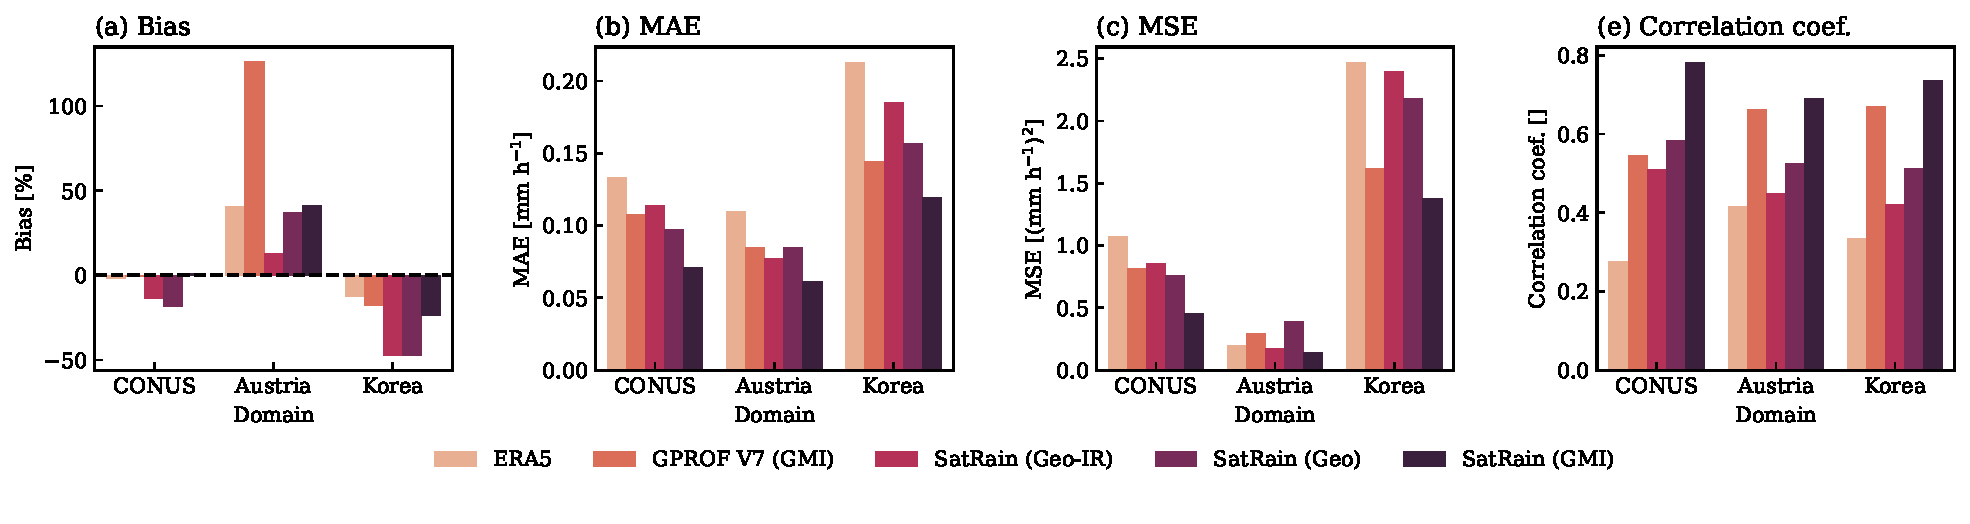
\includegraphics[width=1.0\textwidth]{figures_revised/fig13.pdf}
	\caption{
	  Detection skill for precipitation (first row) and heavy precipitation
	  (second row) for the ERA5 and GPROF V7 baselines and a GMI-based U-Net
	  retrieval trained on the SatRain data. Columns 1 to 3 show the probability
	  of detection (POD), false-alarm rate (FAR), and Heidke Skill Score (HSS)
	  for the deterministic detection. Column 4 shows the area under the
	  precision-recall curve used to assess the probabilistic detection skill.
	}
	\label{fig:precipitation_detection}
\end{figure}


\subsubsection*{Comment 9}
\rc

The baselines deliberately exclude ancillary
data to isolate sensor contributions. It would help to note (in Usage
Notes/Future Directions) that adding ancillary variables often improves
retrieval skill and that SatRain enables those studies (even if you don’t
present them here).

\reply
\paragraph{Author Response}

We extended  Section 5.4 to mention the possibility of studying the impact of
ancillary data using the SatRain dataset.

\paragraph{Changes in Manuscript}

\begin{change}[821]

Furthermore, the
dataset is \DIFdelbegin \DIFdel{ideally suited }\DIFdelend \DIFaddbegin \DIFadd{well-suited }\DIFaddend for tackling broader challenges in global
precipitation retrieval, including the development of sensor-agnostic retrievals
and the mitigation of regional biases. \DIFaddbegin \DIFadd{Additionally, the availability of a broad
range of ancillary data allows studying the impact of the variables on the
retrieval accuracy. }\DIFaddend By providing a common starting point to address these
challenges, SatRain can help guide the community toward more robust,
transferable, and operationally relevant precipitation retrieval systems\DIFaddbegin \DIFadd{.
}


\end{change}

\subsubsection*{Major Comment 10}
\rc

Use consistent forms (e.g., CONUS vs US, ERA5 vs “ERA-5”; NEXRAD capitalization,
and many more).

\reply
\paragraph*{Author Response}

We have revised the manuscript to make the use of abbreviations and acronyms consistent.
